\documentclass[11pt,a4paper]{article}
\usepackage[a4paper,margin=2cm,top=1.8cm,bottom=1.8cm]{geometry}
\usepackage{fontspec}
\setmainfont{texgyretermes}[Extension=.otf,UprightFont=*-regular,BoldFont=*-bold,ItalicFont=*-italic,BoldItalicFont=*-bolditalic]
\setsansfont{texgyreheros}[Extension=.otf,UprightFont=*-regular,BoldFont=*-bold,ItalicFont=*-italic,BoldItalicFont=*-bolditalic]
\usepackage{amsmath,amssymb}
\usepackage{graphicx,booktabs,multirow,array,tabularx}
\usepackage{xcolor}
\usepackage{tikz}
\usetikzlibrary{arrows.meta,positioning,calc}
\usepackage{caption,subcaption}
\usepackage{enumitem}
\usepackage[hidelinks]{hyperref}
\usepackage{titlesec}
\usepackage[section]{placeins}

\definecolor{ptitred}{HTML}{C8102E}
\graphicspath{{../results/figures/}}
\newcommand{\DiceClassicalFull}{0{,}561}
\newcommand{\JacClassicalFull}{0{,}420}
\newcommand{\HdClassicalFull}{40{,}69}
\newcommand{\AsdClassicalFull}{9{,}31}
\newcommand{\VolClassicalFull}{54{,}4}
\newcommand{\DiceUnetFull}{0{,}912}
\newcommand{\JacUnetFull}{0{,}838}
\newcommand{\HdUnetFull}{8{,}22}
\newcommand{\AsdUnetFull}{1{,}71}
\newcommand{\VolUnetFull}{6{,}5}
\newcommand{\DiceSdUnetFull}{0{,}001}
\newcommand{\DiceUnetFew}{0{,}828}
\newcommand{\JacUnetFew}{0{,}716}
\newcommand{\HdUnetFew}{19{,}55}
\newcommand{\AsdUnetFew}{3{,}57}
\newcommand{\VolUnetFew}{17{,}3}
\newcommand{\DiceSdUnetFew}{0{,}013}
\newcommand{\DiceDinoFull}{0{,}902}
\newcommand{\JacDinoFull}{0{,}822}
\newcommand{\HdDinoFull}{11{,}02}
\newcommand{\AsdDinoFull}{1{,}90}
\newcommand{\VolDinoFull}{5{,}9}
\newcommand{\DiceSdDinoFull}{0{,}002}
\newcommand{\DiceDinoFew}{0{,}849}
\newcommand{\JacDinoFew}{0{,}740}
\newcommand{\HdDinoFew}{20{,}55}
\newcommand{\AsdDinoFew}{3{,}50}
\newcommand{\VolDinoFew}{14{,}4}
\newcommand{\DiceSdDinoFew}{0{,}003}
\newcommand{\DiceMriFull}{0{,}908}
\newcommand{\JacMriFull}{0{,}832}
\newcommand{\HdMriFull}{7{,}82}
\newcommand{\AsdMriFull}{1{,}66}
\newcommand{\VolMriFull}{7{,}2}
\newcommand{\DiceSdMriFull}{0{,}001}
\newcommand{\DiceMriFew}{0{,}849}
\newcommand{\JacMriFew}{0{,}744}
\newcommand{\HdMriFew}{13{,}85}
\newcommand{\AsdMriFew}{2{,}80}
\newcommand{\VolMriFew}{11{,}7}
\newcommand{\DiceSdMriFew}{0{,}002}
\newcommand{\DiceConcatFull}{0{,}912}
\newcommand{\JacConcatFull}{0{,}839}
\newcommand{\HdConcatFull}{8{,}13}
\newcommand{\AsdConcatFull}{1{,}64}
\newcommand{\VolConcatFull}{6{,}1}
\newcommand{\DiceSdConcatFull}{0{,}001}
\newcommand{\DiceConcatFew}{0{,}864}
\newcommand{\JacConcatFew}{0{,}762}
\newcommand{\HdConcatFew}{14{,}75}
\newcommand{\AsdConcatFew}{2{,}86}
\newcommand{\VolConcatFew}{9{,}7}
\newcommand{\DiceSdConcatFew}{0{,}003}
\newcommand{\DiceGateFull}{0{,}911}
\newcommand{\JacGateFull}{0{,}838}
\newcommand{\HdGateFull}{7{,}43}
\newcommand{\AsdGateFull}{1{,}60}
\newcommand{\VolGateFull}{6{,}2}
\newcommand{\DiceSdGateFull}{0{,}002}
\newcommand{\DiceGateFew}{0{,}857}
\newcommand{\JacGateFew}{0{,}753}
\newcommand{\HdGateFew}{14{,}67}
\newcommand{\AsdGateFew}{2{,}86}
\newcommand{\VolGateFew}{12{,}4}
\newcommand{\DiceSdGateFew}{0{,}004}
\newcommand{\DiceGateEdgeFull}{0{,}913}
\newcommand{\JacGateEdgeFull}{0{,}840}
\newcommand{\HdGateEdgeFull}{7{,}52}
\newcommand{\AsdGateEdgeFull}{1{,}57}
\newcommand{\VolGateEdgeFull}{6{,}6}
\newcommand{\DiceSdGateEdgeFull}{0{,}001}
\newcommand{\DiceGateEdgeFew}{0{,}862}
\newcommand{\JacGateEdgeFew}{0{,}761}
\newcommand{\HdGateEdgeFew}{14{,}23}
\newcommand{\AsdGateEdgeFew}{2{,}80}
\newcommand{\VolGateEdgeFew}{10{,}6}
\newcommand{\DiceSdGateEdgeFew}{0{,}009}
\newcommand{\DicePpUnetFull}{0{,}914}
\newcommand{\HdPpUnetFull}{6{,}32}
\newcommand{\VolPpUnetFull}{6{,}7}
\newcommand{\DicePpUnetFew}{0{,}841}
\newcommand{\HdPpUnetFew}{12{,}50}
\newcommand{\VolPpUnetFew}{15{,}7}
\newcommand{\DicePpDinoFull}{0{,}908}
\newcommand{\HdPpDinoFull}{7{,}10}
\newcommand{\VolPpDinoFull}{6{,}4}
\newcommand{\DicePpDinoFew}{0{,}861}
\newcommand{\HdPpDinoFew}{14{,}70}
\newcommand{\VolPpDinoFew}{14{,}4}
\newcommand{\DicePpMriFull}{0{,}910}
\newcommand{\HdPpMriFull}{6{,}47}
\newcommand{\VolPpMriFull}{7{,}4}
\newcommand{\DicePpMriFew}{0{,}859}
\newcommand{\HdPpMriFew}{9{,}71}
\newcommand{\VolPpMriFew}{11{,}1}
\newcommand{\DicePpConcatFull}{0{,}915}
\newcommand{\HdPpConcatFull}{6{,}76}
\newcommand{\VolPpConcatFull}{6{,}5}
\newcommand{\DicePpConcatFew}{0{,}876}
\newcommand{\HdPpConcatFew}{9{,}72}
\newcommand{\VolPpConcatFew}{8{,}8}
\newcommand{\DicePpGateFull}{0{,}914}
\newcommand{\HdPpGateFull}{5{,}82}
\newcommand{\VolPpGateFull}{6{,}4}
\newcommand{\DicePpGateFew}{0{,}868}
\newcommand{\HdPpGateFew}{10{,}82}
\newcommand{\VolPpGateFew}{11{,}4}
\newcommand{\DicePpGateEdgeFull}{0{,}915}
\newcommand{\HdPpGateEdgeFull}{6{,}15}
\newcommand{\VolPpGateEdgeFull}{7{,}1}
\newcommand{\DicePpGateEdgeFew}{0{,}872}
\newcommand{\HdPpGateEdgeFew}{10{,}51}
\newcommand{\VolPpGateEdgeFew}{10{,}1}
\newcommand{\PGateVsDinoFull}{{=}0{,}001}
\newcommand{\WinGateVsDinoFull}{18/20}
\newcommand{\DiffGateVsDinoFull}{+0{,}009}
\newcommand{\PGateVsMriFull}{{=}0{,}001}
\newcommand{\WinGateVsMriFull}{16/20}
\newcommand{\DiffGateVsMriFull}{+0{,}003}
\newcommand{\PGateVsConcatFull}{{=}0{,}294}
\newcommand{\WinGateVsConcatFull}{8/20}
\newcommand{\DiffGateVsConcatFull}{-0{,}001}
\newcommand{\PConcatVsDinoFull}{{<}0{,}001}
\newcommand{\WinConcatVsDinoFull}{19/20}
\newcommand{\DiffConcatVsDinoFull}{+0{,}010}
\newcommand{\PMriVsDinoFull}{{=}0{,}036}
\newcommand{\WinMriVsDinoFull}{15/20}
\newcommand{\DiffMriVsDinoFull}{+0{,}006}
\newcommand{\PGateVsUnetFull}{{=}0{,}869}
\newcommand{\WinGateVsUnetFull}{10/20}
\newcommand{\DiffGateVsUnetFull}{-0{,}001}
\newcommand{\PDinoVsUnetFull}{{=}0{,}024}
\newcommand{\WinDinoVsUnetFull}{6/20}
\newcommand{\DiffDinoVsUnetFull}{-0{,}010}
\newcommand{\PMriVsUnetFull}{{=}0{,}231}
\newcommand{\WinMriVsUnetFull}{9/20}
\newcommand{\DiffMriVsUnetFull}{-0{,}004}
\newcommand{\PGateEdgeVsGateFull}{{=}0{,}097}
\newcommand{\WinGateEdgeVsGateFull}{13/20}
\newcommand{\DiffGateEdgeVsGateFull}{+0{,}002}
\newcommand{\PGateEdgeVsUnetFull}{{=}0{,}841}
\newcommand{\WinGateEdgeVsUnetFull}{11/20}
\newcommand{\DiffGateEdgeVsUnetFull}{+0{,}001}
\newcommand{\PGateVsDinoFew}{{=}0{,}154}
\newcommand{\WinGateVsDinoFew}{15/20}
\newcommand{\DiffGateVsDinoFew}{+0{,}008}
\newcommand{\PGateVsMriFew}{{=}0{,}956}
\newcommand{\WinGateVsMriFew}{10/20}
\newcommand{\DiffGateVsMriFew}{+0{,}008}
\newcommand{\PGateVsConcatFew}{{=}0{,}202}
\newcommand{\WinGateVsConcatFew}{8/20}
\newcommand{\DiffGateVsConcatFew}{-0{,}007}
\newcommand{\PConcatVsDinoFew}{{=}0{,}064}
\newcommand{\WinConcatVsDinoFew}{16/20}
\newcommand{\DiffConcatVsDinoFew}{+0{,}015}
\newcommand{\PMriVsDinoFew}{{=}0{,}165}
\newcommand{\WinMriVsDinoFew}{14/20}
\newcommand{\DiffMriVsDinoFew}{-0{,}000}
\newcommand{\PGateVsUnetFew}{{=}0{,}008}
\newcommand{\WinGateVsUnetFew}{16/20}
\newcommand{\DiffGateVsUnetFew}{+0{,}029}
\newcommand{\PDinoVsUnetFew}{{=}0{,}784}
\newcommand{\WinDinoVsUnetFew}{10/20}
\newcommand{\DiffDinoVsUnetFew}{+0{,}021}
\newcommand{\PMriVsUnetFew}{{=}0{,}030}
\newcommand{\WinMriVsUnetFew}{14/20}
\newcommand{\DiffMriVsUnetFew}{+0{,}021}
\newcommand{\PGateEdgeVsGateFew}{{=}0{,}133}
\newcommand{\WinGateEdgeVsGateFew}{13/20}
\newcommand{\DiffGateEdgeVsGateFew}{+0{,}006}
\newcommand{\PGateEdgeVsUnetFew}{{=}0{,}004}
\newcommand{\WinGateEdgeVsUnetFew}{16/20}
\newcommand{\DiffGateEdgeVsUnetFew}{+0{,}034}
\newcommand{\GateInside}{0{,}107}
\newcommand{\GateBoundary}{0{,}296}
\newcommand{\GateNear}{0{,}579}
\newcommand{\GateFar}{0{,}693}
\newcommand{\ClassicalSigma}{2}
\newcommand{\ClassicalK}{1{,}2}
\newcommand{\ClassicalR}{24}
\newcommand{\ParamsUnet}{1{,}94}
\newcommand{\ParamsDino}{0{,}20}
\newcommand{\ParamsGate}{0{,}30}
\newcommand{\ParamsGateEdge}{0{,}30}
\newcommand{\TrainMsDino}{50}
\newcommand{\TrainMsGate}{54}
\newcommand{\TrainMsGateEdge}{76}
\newcommand{\TrainMsUnet}{182}
\newcommand{\InferGate}{10{,}1}
\newcommand{\InferUnet}{0{,}3}
\newcommand{\ErrBand}{64}
\newcommand{\ErrEnds}{39}
\newcommand{\RefBand}{19}
\newcommand{\RefEnds}{19}
\newcommand{\GatePpRawDice}{0{,}911}
\newcommand{\GatePpRawHd}{7{,}43}
\newcommand{\GatePpLccDice}{0{,}912}
\newcommand{\GatePpLccHd}{6{,}24}
\newcommand{\GatePpLccFillDice}{0{,}912}
\newcommand{\GatePpLccFillHd}{6{,}19}
\newcommand{\GatePpLccFillCloseDice}{0{,}914}
\newcommand{\GatePpLccFillCloseHd}{5{,}82}


% Vietnamese captions, no hyphenation inside Vietnamese syllables
\renewcommand{\figurename}{Hình}
\renewcommand{\tablename}{Bảng}
\renewcommand{\refname}{Tài liệu tham khảo}
\renewcommand{\abstractname}{Tóm tắt}
\hyphenpenalty=10000 \exhyphenpenalty=10000 \emergencystretch=3em
\captionsetup{font=small,labelfont=bf,labelsep=period}
\setlist{nosep,leftmargin=1.4em}
\titleformat{\section}{\large\bfseries\color{ptitred}}{\thesection.}{0.5em}{}
\titleformat{\subsection}{\normalsize\bfseries}{\thesubsection.}{0.5em}{}
\titlespacing*{\section}{0pt}{8pt}{4pt}
\titlespacing*{\subsection}{0pt}{6pt}{3pt}
\setlength{\parskip}{3pt}

\newcommand{\RQ}[1]{\textbf{RQ#1}}

\begin{document}

%-------------------------------------------------------------- title block
\begin{center}
{\small HỌC VIỆN CÔNG NGHỆ BƯU CHÍNH VIỄN THÔNG -- KHOA TRÍ TUỆ NHÂN TẠO}\\[2pt]
{\small BÁO CÁO DỰ ÁN MÔN XỬ LÝ ẢNH -- Lựa chọn 2: Dự án xử lý ảnh thực tế}\\[8pt]
{\Large\bfseries\color{ptitred} GateFuse-LA: hợp nhất có cổng đặc trưng tổng quát và đặc trưng chuyên MRI\\[2pt] cho phân đoạn tâm nhĩ trái trên ảnh LGE-MRI}\\[8pt]
{\small Giảng viên: PGS.TS. Phạm Văn Cường \quad|\quad Lớp: \textbf{[Lớp XX]} \quad|\quad Nhóm: \textbf{[Nhóm YY]}}\\[2pt]
{\small Thành viên: [Họ tên SV1], [Họ tên SV2], [Họ tên SV3], [Họ tên SV4], [Họ tên SV5]}\\[2pt]
{\small Mã nguồn: \url{https://github.com/scalliontor/image_processing}}
\end{center}

\begin{abstract}
\noindent
Dự án xây dựng một pipeline xử lý ảnh nhiều bước để phân đoạn khoang tâm nhĩ trái trên ảnh LGE-MRI 3D. Pipeline kết hợp các kỹ thuật cổ điển của học phần (kéo giãn tương phản, lọc Gauss, phân ngưỡng Otsu, toán tử Sobel, phép mở/đóng, thành phần liên thông) với hai mô hình nền tảng được giữ đông cứng: DINOv3 (học trên ảnh tự nhiên) và MRI-CORE (học trên ảnh MRI). Chúng tôi đề xuất \textbf{GateFuse}, một đầu nhẹ (\ParamsGate\,M tham số) học \emph{cổng theo từng điểm ảnh} để ghép hai loại đặc trưng, và biến thể \textbf{D+} có thêm nhánh biên Sobel. Trên 20 khối test của 2018 Atrial Segmentation Challenge (3 seed), với 72 khối huấn luyện D+ đạt Dice \DiceGateEdgeFull{} (\DicePpGateEdgeFull{} sau hậu xử lý), ngang U-Net học từ đầu (\DiceUnetFull) và vượt xa pipeline cổ điển thuần (\DiceClassicalFull). Khi chỉ có 8 khối có nhãn, các đầu dùng đặc trưng nền tảng vượt U-Net khoảng 3 điểm Dice (D+ \DiceGateEdgeFew{} so với \DiceUnetFew, $p\PGateEdgeVsUnetFew$). Đặc trưng chuyên MRI tốt hơn đặc trưng tổng quát, ghép hai loại tốt hơn từng loại riêng, và bản đồ cổng cho thấy mô hình dựa vào MRI-CORE bên trong tâm nhĩ ($g=\GateInside$), dựa vào DINOv3 ở vùng ngữ cảnh ($g=\GateFar$). Hậu xử lý hình thái giảm HD95 từ 17\% đến 36\%.
\end{abstract}

%-------------------------------------------------------------- 1
\section{Bài toán}
\textbf{Định nghĩa.} Cho một khối ảnh cộng hưởng từ tăng cường muộn gadolinium (LGE-MRI) của tim, gồm 88 lát cắt ngang kích thước $h\times w$ (đã cắt quanh vùng tâm nhĩ), cần sinh ra một \emph{mặt nạ nhị phân 3D} đánh dấu các voxel thuộc khoang tâm nhĩ trái (left atrium, LA). Mặt nạ LA là đầu vào của việc đo thể tích nhĩ, dựng mô hình giải phẫu và định vị sẹo xơ hoá trước khi đốt điện điều trị rung nhĩ. Phân đoạn thủ công một khối mất nhiều giờ và phụ thuộc người vẽ.

\textbf{Đầu vào / đầu ra.} Đầu vào là khối xám $h\times w\times 88$ (voxel đẳng hướng 0.625\,mm). Đầu ra là mặt nạ cùng kích thước. Chất lượng được đo bằng Dice, Jaccard, khoảng cách Hausdorff 95\% (HD95), khoảng cách bề mặt trung bình (ASD) và sai số thể tích tâm nhĩ.

\textbf{Khó khăn cốt lõi.}
\begin{itemize}
\item \emph{Cường độ không phân biệt được}: máu trong LA sáng ngang tĩnh mạch phổi, động mạch chủ và các buồng tim lân cận, nên phân ngưỡng cường độ đơn thuần luôn ``tràn'' sang cấu trúc khác.
\item \emph{Biên yếu và nhiễu}: tương phản LGE thấp, cường độ không đồng đều giữa các ca và giữa các lát.
\item \emph{Hình dạng biến thiên}: tĩnh mạch phổi và tiểu nhĩ trái mảnh, số nhánh khác nhau giữa bệnh nhân.
\item \emph{Ít nhãn}: nhãn do chuyên gia vẽ tay theo từng voxel nên rất đắt; một phương pháp tốt phải dùng ít nhãn mà vẫn ổn định.
\end{itemize}

\textbf{Ý tưởng và câu hỏi nghiên cứu.} Các mô hình nền tảng (foundation model) cho đặc trưng ảnh mạnh mà không cần học lại. Có hai loại: mô hình \emph{tổng quát} như DINOv3 \cite{dinov3} học trên khoảng 1,7 tỷ ảnh tự nhiên (giỏi hình dạng, biên vật thể nhưng chưa thấy ảnh MRI), và mô hình \emph{chuyên MRI} như MRI-CORE \cite{mricore} học trên khoảng 6 triệu lát MRI (quen tương phản và nhiễu MRI nhưng nhỏ hơn, và trong mô tả dữ liệu tiền huấn luyện không nhắc tới tim). Chúng tôi đề xuất \textbf{GateFuse}: giữ đông cứng cả hai encoder và học một \emph{cổng theo từng điểm ảnh} quyết định nên tin đặc trưng nào; biến thể \textbf{D+} bổ sung một nhánh biên Sobel ở độ phân giải đầy đủ để bù độ thô của token ViT. Dự án trả lời:
\RQ{1}: đặc trưng chuyên MRI có tốt hơn đặc trưng tổng quát cho LA trên LGE-MRI không? \;
\RQ{2}: ghép hai loại đặc trưng có bổ sung cho nhau không, và ghép có cổng có hơn ghép nối đơn giản không? \;
\RQ{3}: cổng tin encoder nào, ở vùng giải phẫu nào? \;
\RQ{4}: khi chỉ có 8 khối có nhãn thì kết luận có thay đổi không? \;
\RQ{5}: hậu xử lý hình thái học (chương 7) đóng góp bao nhiêu?

%-------------------------------------------------------------- 2
\section{Các nghiên cứu liên quan}
Bộ dữ liệu và thách thức phân đoạn LA trên LGE-MRI được tổng kết trong \cite{xiong2021}; bản cắt sẵn 100 khối của \cite{uamt} trở thành chuẩn so sánh cho học bán giám sát. Với mô hình nền tảng, AdaDINO-LA \cite{adadino} so sánh các cách tinh chỉnh DINOv2 \cite{dinov2} cho LA (Dice $\approx$0.91, thua nnU-Net $\approx$0.93); Kundu và cs.\ \cite{kundu2025} dùng DINOv2 với decoder kiểu U-Net. Với DINOv3, \cite{liu2025dinov3med} cho thấy đây là một mốc so sánh mạnh trong ảnh y tế nhưng không phải lúc nào mô hình lớn hơn hay độ phân giải cao hơn cũng tốt hơn. MRI-CORE \cite{mricore} huấn luyện DINOv2 trên dữ liệu MRI (khởi tạo từ SAM \cite{sam}) và báo cáo lợi thế lớn khi ít nhãn. Việc ghép đặc trưng DINOv2 với SAM/SAM2 đã được thử ở \cite{dsunet}; theo hiểu biết của chúng tôi, chưa có nghiên cứu ghép DINOv3 với một mô hình nền tảng MRI cho bài toán LA.

%-------------------------------------------------------------- 3
\section{Dữ liệu}
\begin{itemize}
\item \textbf{Nguồn}: 100 khối LGE-MRI có nhãn của \emph{2018 Atrial Segmentation Challenge} \cite{xiong2021}, bản phân phối công khai dạng \texttt{.h5} trong kho mã UA-MT \cite{uamt}. Nhãn khoang LA do chuyên gia vẽ tay theo từng voxel (đây là nhãn gốc của cuộc thi, nhóm không gán nhãn thêm).
\item \textbf{Định dạng}: mỗi khối đã được cắt quanh tâm nhĩ (kích thước mặt phẳng từ $148\times132$ đến $244\times160$, 88 lát), cường độ đã chuẩn hoá $z$-score. Lưu ý: vùng cắt được lấy từ hộp bao của nhãn (quy ước của \cite{uamt}), nên bài toán định vị đã được đơn giản hoá cho \emph{mọi} phương pháp.
\item \textbf{Chia tập theo ca bệnh} (không chia theo lát để tránh rò rỉ): giữ nguyên danh sách 80 train / 20 test chính thức của \cite{uamt}; 8 khối cuối của danh sách train làm tập kiểm định (validation). Kết quả: \textbf{72 khối huấn luyện (6\,336 lát), 8 khối validation (704 lát), 20 khối test (1\,760 lát, trong đó 1\,231 lát có tâm nhĩ)}, vượt xa yêu cầu $\ge$50 ảnh đánh giá.
\item \textbf{Chế độ ít nhãn}: chỉ dùng 8 khối đầu danh sách train (10\%, giống thiết lập bán giám sát phổ biến).
\item \textbf{Thống kê nhãn}: thể tích tâm nhĩ 54,7\,$\pm$\,21,1\,mL (18,6--132,1\,mL); 67\% số lát của mỗi khối có tâm nhĩ; tâm nhĩ chỉ chiếm khoảng 9\% số voxel của vùng cắt, nên hàm mất mát có thêm thành phần Dice để chống mất cân bằng lớp.
\end{itemize}

%-------------------------------------------------------------- 4
\section{Phương pháp}
\begin{figure}[t]
\centering
\resizebox{\linewidth}{!}{% Pipeline diagram shared by the report and the slides (needs tikz + arrows.meta, positioning)
\begin{tikzpicture}[
  font=\sffamily\scriptsize, >=Stealth, node distance=3mm and 4mm,
  box/.style={draw=black!55, rounded corners=2pt, align=center, inner sep=3pt, minimum height=9mm, fill=white},
  stage/.style={box, fill=ptitred!8},
  enc/.style={box, minimum width=27mm},
  arr/.style={->, thick, black!65},
  lab/.style={font=\sffamily\tiny, text=black!60}]
  \node[stage] (in) {Khối LGE-MRI\\$h\times w\times 88$};
  \node[stage, right=of in] (pre) {Tiền xử lý (ch.\,2--3)\\cắt percentile 0.5--99.5\\min--max theo lát\\đệm 256, phóng $\times2$};
  \node[enc, right=6mm of pre, yshift=7mm, fill=blue!7] (dino) {DINOv3 ViT-B/16\\(đông cứng, ảnh tự nhiên)};
  \node[enc, right=6mm of pre, yshift=-7mm, fill=orange!10] (mri) {MRI-CORE ViT-B/16\\(đông cứng, 6\,tr lát MRI)};
  \node[box, right=13mm of dino] (pd) {chiếu $1{\times}1$\\$P_D$};
  \node[box, right=13mm of mri] (pm) {chiếu $1{\times}1$\\$P_M$};
  \path (pd.east) -- (pm.east) coordinate[midway] (mid);
  \node[box, right=6mm of mid, fill=green!8] (gate) {Cổng học được\\$g=\sigma(\mathrm{conv}[P_D,P_M])$\\$F=g P_D+(1-g)P_M$};
  \node[box, right=of gate] (dec) {Decoder\\$32\to256$};
  \node[stage, right=of dec] (post) {Hậu xử lý (ch.\,7)\\ngưỡng 0.5\\TPLT 3D lớn nhất\\lấp lỗ};
  \node[box, below=4mm of post] (out) {Mặt nạ 3D\\Dice, Jaccard\\HD95, ASD};
  \node[box, dashed, fill=violet!6, below=9mm of gate] (det) {Nhánh chi tiết (D+)\\ảnh + gradient Sobel (ch.\,5)\\2 lớp conv ở $256{\times}256$};
  \draw[arr] (in) -- (pre);
  \draw[arr] (pre.east) -- ++(3mm,0) |- (dino.west);
  \draw[arr] (pre.east) -- ++(3mm,0) |- (mri.west);
  \draw[arr] (dino) -- node[above, lab]{$768{\times}32{\times}32$} (pd);
  \draw[arr] (mri) -- node[below, lab]{$768{\times}32{\times}32$} (pm);
  \draw[arr] (pd.east) -- ++(2mm,0) |- (gate.west);
  \draw[arr] (pm.east) -- ++(2mm,0) |- (gate.west);
  \draw[arr] (gate) -- (dec);
  \draw[arr] (dec) -- (post);
  \draw[arr] (post) -- (out);
  \draw[arr, dashed] (pre.south) |- (det.west);
  \draw[arr, dashed] (det.east) -| node[pos=0.8, right, lab]{ghép} (dec.south);
\end{tikzpicture}
}
\caption{Pipeline GateFuse-LA. Hai encoder ViT-B/16 đông cứng nhận cùng một ảnh; chỉ phần chiếu, cổng và decoder (khoảng 0,3\,M tham số) được huấn luyện. Nhánh nét đứt chỉ có ở biến thể D+. TPLT: thành phần liên thông.}
\label{fig:pipeline}
\end{figure}

\subsection{Tiền xử lý (chương 2--3)}
Mỗi lát được \emph{kéo giãn tương phản}: cắt cường độ tại phân vị 0,5\% và 99,5\% rồi đưa về $[0,1]$ bằng min--max. Lý do: loại các điểm quá sáng/tối hiếm gặp (nhiễu, mỡ tăng tín hiệu) trước khi chuẩn hoá; chuẩn hoá theo lát là cách MRI-CORE dùng khi tiền huấn luyện. Lát được \emph{đệm số 0} vào khung $256\times256$ (không co ảnh, nên nhãn giữ nguyên độ phân giải gốc), rồi phóng $\times2$ bằng nội suy song tuyến lên $512\times512$ để mỗi ô $16\times16$ của ViT ứng với $8\times8$ điểm ảnh gốc; ảnh xám được nhân thành 3 kênh và chuẩn hoá theo trung bình/độ lệch ImageNet (cả hai encoder đều được huấn luyện với chuẩn hoá này).

\subsection{Hai encoder nền tảng đông cứng}
\textbf{DINOv3 ViT-B/16} \cite{dinov3} (86\,M tham số, mã hoá vị trí RoPE, 4 token thanh ghi) học tự giám sát trên LVD-1689M. \textbf{MRI-CORE ViT-B/16} \cite{mricore} là một ViT kiểu DINOv2 học trên dữ liệu MRI; chúng tôi nạp checkpoint \emph{teacher} chính thức vào ViT-B/16 chuẩn của thư viện \texttt{timm} và nội suy lưới vị trí $14\times14\to32\times32$. Với ảnh $512\times512$, mỗi encoder trả về bản đồ token $768\times32\times32$ (lấy sau LayerNorm cuối). Vì encoder đông cứng và không dùng tăng cường dữ liệu, đặc trưng của 8\,800 lát được tính \emph{một lần} và lưu lại (khoảng 10 phút/encoder trên Apple M2 Pro), nên mọi thí nghiệm phía sau chỉ huấn luyện phần đầu nhẹ.

\subsection{Đầu ghép và decoder}
Mỗi đặc trưng đi qua phép chiếu $1{\times}1$ (Conv--BN--ReLU) về 128 kênh: $P_D$ (DINOv3), $P_M$ (MRI-CORE). Bốn cấu hình dùng \emph{chung} decoder và chỉ khác cách tạo $F$:
\begin{itemize}
\item \textbf{A} (chỉ DINOv3): $F=P_D$; \quad \textbf{B} (chỉ MRI-CORE): $F=P_M$;
\item \textbf{C} (ghép nối): $F=\mathrm{ReLU}(\mathrm{BN}(W_{1\times1}[P_D;P_M]))$;
\item \textbf{D} (GateFuse, đề xuất): $g=\sigma(W_{3\times3}*[P_D;P_M])\in[0,1]^{32\times32}$, \; $F=g\odot P_D+(1-g)\odot P_M$. Trọng số cổng khởi tạo bằng 0 nên ban đầu $g=0{,}5$ ở mọi nơi.
\item \textbf{D+} (GateFuse + nhánh chi tiết): mỗi token ViT phủ $8\times8$ điểm ảnh gốc nên biên bị thô. D+ thêm một nhánh ở độ phân giải đầy đủ $256\times256$ nhận ảnh $I$ và độ lớn gradient Sobel $|\nabla I|=\sqrt{(S_x*I)^2+(S_y*I)^2}$ (chương 5), qua 2 lớp Conv $3{\times}3$ (16 kênh), rồi ghép vào tầng cuối của decoder. Nhánh này chỉ thêm khoảng 4 nghìn tham số.
\end{itemize}
Decoder gồm 3 khối (phóng $\times2$ song tuyến, Conv $3{\times}3$--BN--ReLU; $128\to64\to32\to16$ kênh) đưa $32\times32$ lên $256\times256$, rồi Conv $3{\times}3$ và Conv $1{\times}1$ ra logit. Hàm mất mát là $0{,}5\,\mathrm{BCE}+0{,}5\,(1-\mathrm{Dice}_{\text{mềm}})$.

\subsection{Hậu xử lý hình thái (chương 7)}
Xác suất được cắt bỏ phần đệm, xếp lại thành khối 3D và lấy ngưỡng 0,5. Vì mạng dự đoán từng lát độc lập, khối có thể chứa đốm rời và lỗ nhỏ. Ba bước được so sánh: (i) giữ \emph{thành phần liên thông 3D lớn nhất} (liên thông 26); (ii) \emph{lấp lỗ} trong từng lát; (iii) \emph{phép đóng} với phần tử cấu trúc hình cầu bán kính 1 trước khi lấp lỗ.

\subsection{Phương pháp đối chứng}
\textbf{Cổ điển (không học)}: lọc Gauss 3D độ lệch $\sigma$ (chương 3) $\to$ ngưỡng Otsu toàn cục nhân hệ số $k$ (chương 5) $\to$ phép mở với phần tử hình thoi bán kính $r$ để cắt các cầu nối mảnh giữa LA và tĩnh mạch phổi/động mạch chủ (chương 7) $\to$ giữ thành phần liên thông nằm nhiều nhất trong nửa trung tâm khối $\to$ đóng và lấp lỗ. Bộ $(\sigma,k,r)$ được dò lưới trên 24 khối train/validation (không dùng tập test); bộ tốt nhất là $\sigma=\ClassicalSigma$, $k=\ClassicalK$, $r=\ClassicalR$.
\textbf{U-Net 2D} \cite{unet} học từ đầu trên ảnh (4 lần lấy mẫu xuống, 16 kênh gốc như V-Net của \cite{uamt}, \ParamsUnet\,M tham số), cùng hàm mất mát, cùng số vòng lặp: đại diện cho cách làm không dùng tiền huấn luyện.

\begin{table}[t]
\centering\small
\caption{Kiến thức học phần được sử dụng (theo cách phân chương của học phần, tham khảo \cite{gonzalez}).}
\label{tab:chapters}
\begin{tabularx}{\linewidth}{lXc}
\toprule
Bước & Kỹ thuật & Chương\\
\midrule
Tiền xử lý & cắt phân vị + kéo giãn min--max (biến đổi cường độ); đệm, nội suy song tuyến & 2, 3\\
Đối chứng cổ điển & lọc Gauss 3D làm trơn nhiễu & 3\\
Đối chứng cổ điển & phân ngưỡng Otsu toàn cục \cite{otsu} & 5\\
Biến thể D+ & toán tử Sobel, độ lớn gradient (phát hiện biên) & 5\\
Đối chứng \& hậu xử lý & phép mở, phép đóng, thành phần liên thông, lấp lỗ & 7\\
Phân tích đặc trưng & PCA trên đặc trưng token để trực quan hoá biểu diễn & 8\\
Đánh giá & Dice/Jaccard; HD95, ASD qua biến đổi khoảng cách trên biên & 5, 7\\
\bottomrule
\end{tabularx}
\end{table}

%-------------------------------------------------------------- 5
\section{Thiết lập thực nghiệm}
Mọi cấu hình học dùng AdamW (lr $10^{-3}$, weight decay $10^{-4}$, khởi động tuyến tính 100 vòng rồi giảm theo cosin), batch 16, \textbf{4\,000 vòng} với 72 khối ($\approx$10 epoch) và \textbf{2\,000 vòng} với 8 khối ($\approx$45 epoch). Cứ 250 (hoặc 200) vòng, mô hình được chấm Dice 3D trên 8 khối validation (ngưỡng 0,5, không hậu xử lý); checkpoint tốt nhất được dùng cho tập test. Mỗi cấu hình chạy với \textbf{3 seed} (0, 1, 2); bảng báo cáo trung bình $\pm$ độ lệch chuẩn \emph{giữa các seed} của trung bình 20 ca test. Không dùng tăng cường dữ liệu cho mọi cấu hình, để so sánh công bằng. Độ đo tính trên khối 3D ở độ phân giải gốc; HD95 và ASD tính bằng voxel (1 voxel = 0,625\,mm); ngoài ra báo cáo \emph{sai số thể tích tâm nhĩ} $|\Delta V|=|V_{\text{dự đoán}}-V_{\text{nhãn}}|/V_{\text{nhãn}}$ (\%) vì đo thể tích nhĩ là ứng dụng lâm sàng trực tiếp của mặt nạ. So sánh từng cặp phương pháp dùng kiểm định Wilcoxon có dấu trên Dice từng ca (trung bình 3 seed). Toàn bộ chạy trên một Apple M2 Pro (GPU tích hợp, MPS), 32\,GB RAM.

%-------------------------------------------------------------- 6
\section{Kết quả}
\begin{figure}[t]
\centering
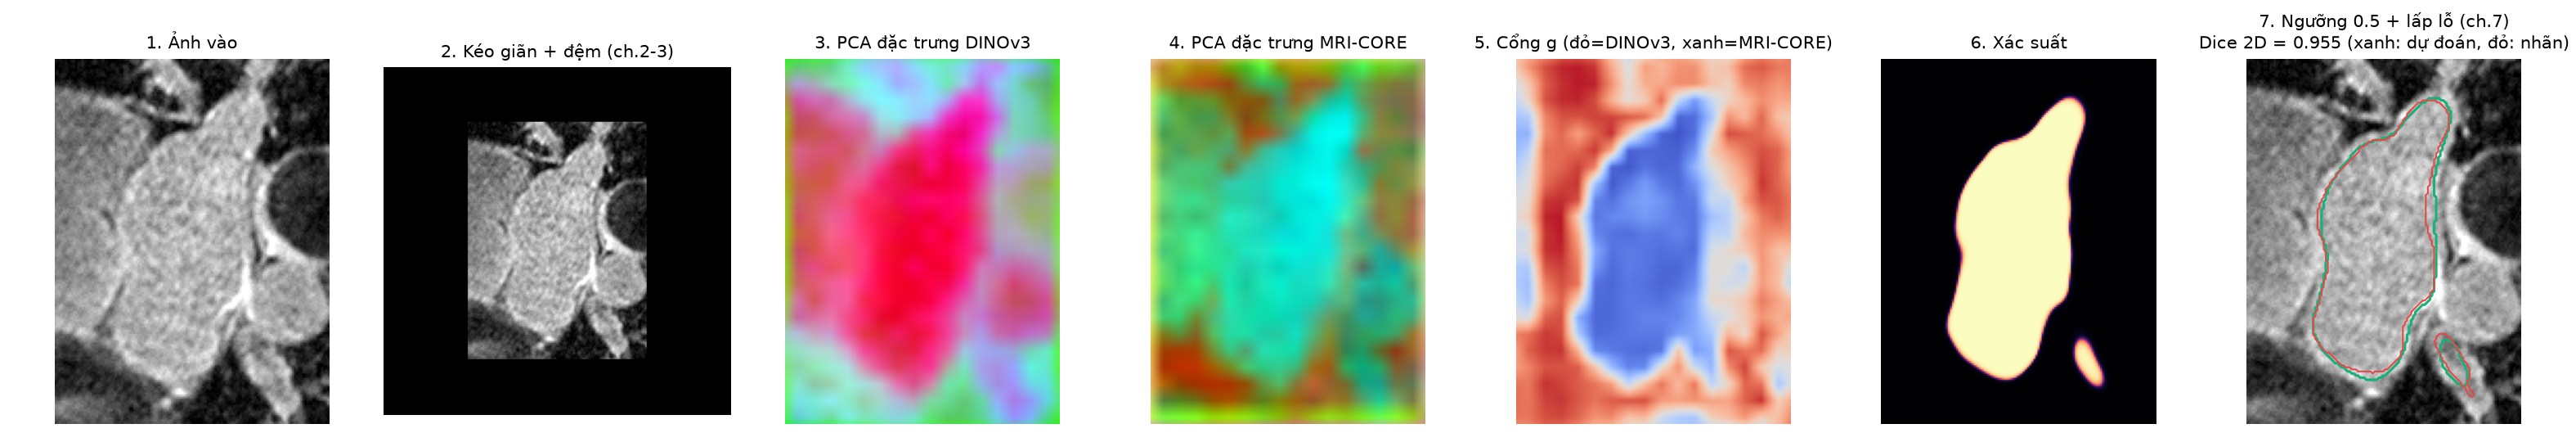
\includegraphics[width=\linewidth]{demo_UPT6DX9I_z52_img.png}
\caption{Pipeline chạy trên một lát test thật (ca UPT6DX9I, lát 52): (1) ảnh vào; (2) sau kéo giãn tương phản và đệm; (3--4) ba thành phần PCA đầu của token DINOv3 và MRI-CORE (đã trừ trung bình theo vị trí ô) -- cả hai đều tách khoang tâm nhĩ thành một vùng riêng dù chưa từng được huấn luyện cho LA; (5) cổng $g$; (6) xác suất; (7) kết quả (xanh) so với nhãn (đỏ).}
\label{fig:demo}
\end{figure}

\subsection{So sánh chính với 72 khối có nhãn}
Bảng~\ref{tab:main} và Hình~\ref{fig:box} tổng hợp kết quả. \textbf{Pipeline cổ điển} chỉ đạt Dice \DiceClassicalFull{} dù đã dò 286 bộ tham số: phép mở đủ lớn để cắt tĩnh mạch phổi ($r=\ClassicalR$) cũng bào mòn tâm nhĩ, và ở một ca bước chọn thành phần trung tâm chọn nhầm cấu trúc (Dice 0, Hình~\ref{fig:qual}). Đây là minh chứng định lượng cho khó khăn ``cường độ không phân biệt được''. Mọi phương pháp học đều đạt Dice trên 0,90.

\textbf{RQ1.} Đặc trưng chuyên MRI tốt hơn đặc trưng tổng quát: B đạt \DiceMriFull{} so với \DiceDinoFull{} của A (thắng \WinMriVsDinoFull{} ca, $p\PMriVsDinoFull$), và tốt hơn rõ ở biên (HD95 \HdMriFull{} so với \HdDinoFull{} voxel).
\textbf{RQ2.} Ghép hai encoder tốt hơn từng encoder: GateFuse (\DiceGateFull) hơn MRI-CORE ở \WinGateVsMriFull{} ca ($p\PGateVsMriFull$) và hơn DINOv3 ở \WinGateVsDinoFull{} ca ($p\PGateVsDinoFull$). Ghép có cổng và ghép nối cho Dice tương đương (\DiceGateFull{} và \DiceConcatFull, $p\PGateVsConcatFull$), nhưng cổng có HD95 thấp hơn (\HdGateFull{} so với \HdConcatFull{} voxel) và cho bản đồ giải thích được (mục~6.4).
\textbf{U-Net} học từ đầu với 72 khối đạt \DiceUnetFull, ngang các đầu ghép (so với GateFuse $p\PGateVsUnetFull$): khi đủ nhãn, một mạng tích chập học đầu--cuối ở độ phân giải đầy đủ bù được lợi thế của đặc trưng nền tảng. \textbf{D+} có Dice cao nhất (\DiceGateEdgeFull) và độ lệch giữa các seed nhỏ nhất, nhưng khác biệt với GateFuse ($p\PGateEdgeVsGateFull$) và U-Net ($p\PGateEdgeVsUnetFull$) chưa có ý nghĩa thống kê. Sai số thể tích tâm nhĩ của các phương pháp học khoảng 6--7\%, so với \VolClassicalFull\% của pipeline cổ điển.

\begin{table}[t]
\centering\small
\caption{Kết quả trên 20 khối test khi huấn luyện với 72 khối (ngưỡng 0,5, chưa hậu xử lý). Trung bình $\pm$ độ lệch chuẩn qua 3 seed; phương pháp cổ điển là tất định. In đậm: tốt nhất mỗi cột.}
\label{tab:main}
\resizebox{\linewidth}{!}{\begin{tabular}{lrccccc}
\toprule
Phương pháp & Tham số học & Dice $\uparrow$ & Jaccard $\uparrow$ & HD95 (vx) $\downarrow$ & ASD (vx) $\downarrow$ & $|\Delta V|$ (\%) $\downarrow$\\
\midrule
Cổ điển (Otsu + hình thái) & 0 & 0{,}561 & 0{,}420 & 40{,}69 & 9{,}31 & 54{,}4\\
U-Net 2D (từ đầu) & 1{,}94\,M & 0{,}912{\scriptsize$\pm$0{,}001} & 0{,}838{\scriptsize$\pm$0{,}002} & 8{,}22{\scriptsize$\pm$1{,}01} & 1{,}71{\scriptsize$\pm$0{,}07} & 6{,}5{\scriptsize$\pm$0{,}3}\\
A: DINOv3 & 0{,}20\,M & 0{,}902{\scriptsize$\pm$0{,}002} & 0{,}822{\scriptsize$\pm$0{,}004} & 11{,}02{\scriptsize$\pm$0{,}97} & 1{,}90{\scriptsize$\pm$0{,}10} & \textbf{5{,}9{\scriptsize$\pm$0{,}2}}\\
B: MRI-CORE & 0{,}20\,M & 0{,}908{\scriptsize$\pm$0{,}001} & 0{,}832{\scriptsize$\pm$0{,}001} & 7{,}82{\scriptsize$\pm$0{,}16} & 1{,}66{\scriptsize$\pm$0{,}02} & 7{,}2{\scriptsize$\pm$0{,}5}\\
C: Ghép nối & 0{,}33\,M & 0{,}912{\scriptsize$\pm$0{,}001} & 0{,}839{\scriptsize$\pm$0{,}002} & 8{,}13{\scriptsize$\pm$0{,}56} & 1{,}64{\scriptsize$\pm$0{,}06} & 6{,}1{\scriptsize$\pm$0{,}9}\\
\textbf{D: GateFuse (đề xuất)} & 0{,}30\,M & 0{,}911{\scriptsize$\pm$0{,}002} & 0{,}838{\scriptsize$\pm$0{,}004} & \textbf{7{,}43{\scriptsize$\pm$1{,}03}} & 1{,}60{\scriptsize$\pm$0{,}10} & 6{,}2{\scriptsize$\pm$0{,}4}\\
\textbf{D+: GateFuse + nhánh Sobel} & 0{,}30\,M & \textbf{0{,}913{\scriptsize$\pm$0{,}001}} & \textbf{0{,}840{\scriptsize$\pm$0{,}001}} & 7{,}52{\scriptsize$\pm$0{,}48} & \textbf{1{,}57{\scriptsize$\pm$0{,}03}} & 6{,}6{\scriptsize$\pm$0{,}8}\\
\bottomrule
\end{tabular}}
\end{table}

\begin{figure}[t]
\centering
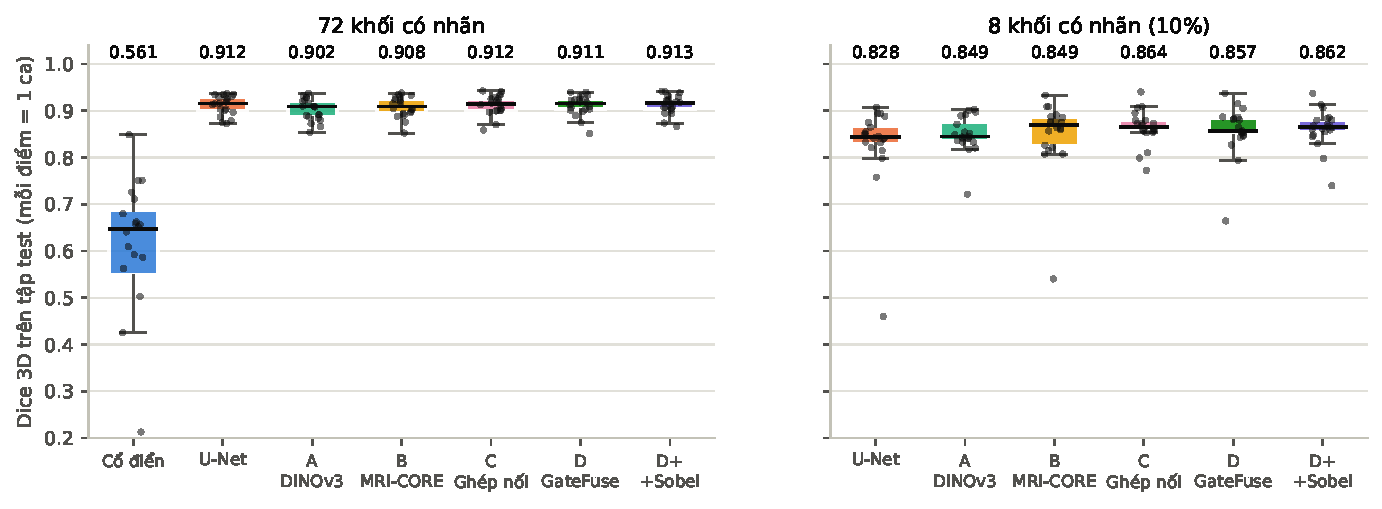
\includegraphics[width=\linewidth,height=5.6cm,keepaspectratio]{dice_boxplot.pdf}
\caption{Dice 3D của từng ca test (trung bình 3 seed). Số phía trên mỗi hộp là Dice trung bình.}
\label{fig:box}
\end{figure}

\subsection{Khi chỉ có 8 khối có nhãn}
Bảng~\ref{tab:few}, Hình~\ref{fig:few} và Bảng~\ref{tab:wilcoxon}. Khi chỉ có 8 khối có nhãn, \textbf{U-Net giảm mạnh nhất} (\DiceUnetFull{} $\to$ \DiceUnetFew) và dao động nhiều giữa các seed ($\pm$\DiceSdUnetFew), trong khi các đầu dùng đặc trưng nền tảng giữ được 0,85--0,86. GateFuse hơn U-Net \DiffGateVsUnetFew{} Dice (thắng \WinGateVsUnetFew{} ca, $p\PGateVsUnetFew$), D+ hơn \DiffGateEdgeVsUnetFew{} ($p\PGateEdgeVsUnetFew$); HD95 giảm từ \HdUnetFew{} xuống khoảng 14 voxel và sai số thể tích từ \VolUnetFew\% xuống \VolGateEdgeFew\% (D+). Ở chế độ này MRI-CORE và DINOv3 có Dice bằng nhau (\DiceMriFew{} và \DiceDinoFew) nhưng MRI-CORE cho biên tốt hơn nhiều (HD95 \HdMriFew{} so với \HdDinoFew). Ghép nối đạt Dice cao nhất (\DiceConcatFew); khác biệt giữa C, D và D+ không có ý nghĩa thống kê.

\begin{table}[t]
\centering\small
\caption{Kết quả trên 20 khối test khi chỉ huấn luyện với 8 khối có nhãn (cùng định dạng Bảng~\ref{tab:main}).}
\label{tab:few}
\resizebox{\linewidth}{!}{\begin{tabular}{lrccccc}
\toprule
Phương pháp & Tham số học & Dice $\uparrow$ & Jaccard $\uparrow$ & HD95 (vx) $\downarrow$ & ASD (vx) $\downarrow$ & $|\Delta V|$ (\%) $\downarrow$\\
\midrule
U-Net 2D (từ đầu) & 1{,}94\,M & 0{,}828{\scriptsize$\pm$0{,}013} & 0{,}716{\scriptsize$\pm$0{,}024} & 19{,}55{\scriptsize$\pm$7{,}29} & 3{,}57{\scriptsize$\pm$0{,}82} & 17{,}3{\scriptsize$\pm$3{,}5}\\
A: DINOv3 & 0{,}20\,M & 0{,}849{\scriptsize$\pm$0{,}003} & 0{,}740{\scriptsize$\pm$0{,}005} & 20{,}55{\scriptsize$\pm$1{,}58} & 3{,}50{\scriptsize$\pm$0{,}19} & 14{,}4{\scriptsize$\pm$3{,}9}\\
B: MRI-CORE & 0{,}20\,M & 0{,}849{\scriptsize$\pm$0{,}002} & 0{,}744{\scriptsize$\pm$0{,}001} & \textbf{13{,}85{\scriptsize$\pm$1{,}31}} & 2{,}80{\scriptsize$\pm$0{,}13} & 11{,}7{\scriptsize$\pm$0{,}8}\\
C: Ghép nối & 0{,}33\,M & \textbf{0{,}864{\scriptsize$\pm$0{,}003}} & \textbf{0{,}762{\scriptsize$\pm$0{,}006}} & 14{,}75{\scriptsize$\pm$1{,}86} & 2{,}86{\scriptsize$\pm$0{,}19} & \textbf{9{,}7{\scriptsize$\pm$0{,}5}}\\
\textbf{D: GateFuse (đề xuất)} & 0{,}30\,M & 0{,}857{\scriptsize$\pm$0{,}004} & 0{,}753{\scriptsize$\pm$0{,}006} & 14{,}67{\scriptsize$\pm$1{,}31} & 2{,}86{\scriptsize$\pm$0{,}10} & 12{,}4{\scriptsize$\pm$2{,}0}\\
\textbf{D+: GateFuse + nhánh Sobel} & 0{,}30\,M & 0{,}862{\scriptsize$\pm$0{,}009} & 0{,}761{\scriptsize$\pm$0{,}013} & 14{,}23{\scriptsize$\pm$0{,}90} & \textbf{2{,}80{\scriptsize$\pm$0{,}08}} & 10{,}6{\scriptsize$\pm$1{,}8}\\
\bottomrule
\end{tabular}}
\end{table}

\begin{figure}[t]
\centering
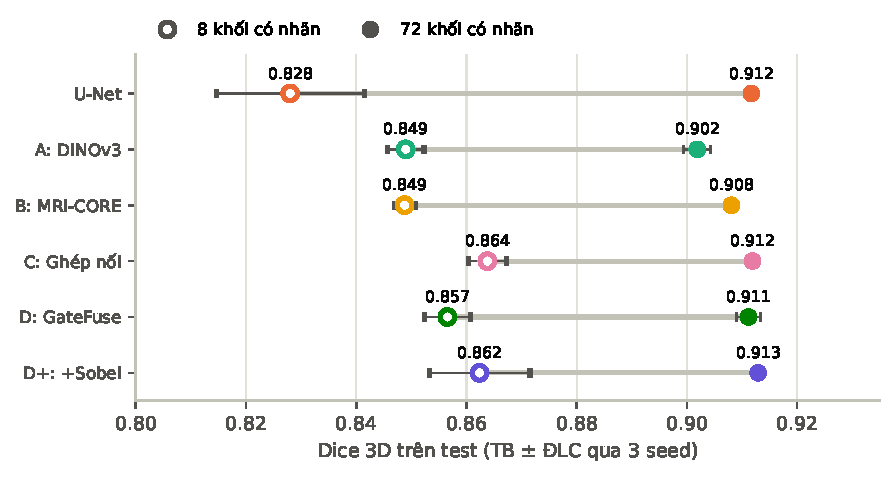
\includegraphics[width=0.72\linewidth]{label_efficiency.pdf}
\caption{Dice của từng cấu hình khi huấn luyện với 8 khối (chấm rỗng) và 72 khối (chấm đặc); thanh ngang là độ lệch chuẩn qua 3 seed. Đoạn nối càng dài, mô hình càng phụ thuộc vào lượng nhãn.}
\label{fig:few}
\end{figure}

\begin{table}[t]
\centering\small
\caption{Kiểm định Wilcoxon có dấu trên Dice từng ca (20 ca, trung bình 3 seed). $\Delta$Dice: chênh lệch trung bình (vế trái trừ vế phải); thắng: số ca vế trái tốt hơn; in đậm: $p<0{,}05$.}
\label{tab:wilcoxon}
\begin{tabular}{lrrrrrr}
\toprule
 & \multicolumn{3}{c}{72 khối có nhãn} & \multicolumn{3}{c}{8 khối có nhãn}\\
\cmidrule(lr){2-4}\cmidrule(lr){5-7}
So sánh & $\Delta$Dice & thắng & $p$ & $\Delta$Dice & thắng & $p$\\
\midrule
MRI-CORE vs DINOv3 & +0{,}0062 & 15/20 & \textbf{0{,}036} & -0{,}0002 & 14/20 & 0{,}165\\
Ghép nối vs DINOv3 & +0{,}0100 & 19/20 & \textbf{$<$0{,}001} & +0{,}0148 & 16/20 & 0{,}064\\
GateFuse vs DINOv3 & +0{,}0093 & 18/20 & \textbf{0{,}001} & +0{,}0076 & 15/20 & 0{,}154\\
GateFuse vs MRI-CORE & +0{,}0031 & 16/20 & \textbf{0{,}001} & +0{,}0078 & 10/20 & 0{,}956\\
GateFuse vs Ghép nối & -0{,}0007 & 8/20 & 0{,}294 & -0{,}0072 & 8/20 & 0{,}202\\
D+ vs GateFuse & +0{,}0017 & 13/20 & 0{,}097 & +0{,}0058 & 13/20 & 0{,}133\\
GateFuse vs U-Net & -0{,}0005 & 10/20 & 0{,}869 & +0{,}0285 & 16/20 & \textbf{0{,}008}\\
D+ vs U-Net & +0{,}0012 & 11/20 & 0{,}841 & +0{,}0344 & 16/20 & \textbf{0{,}004}\\
\bottomrule
\end{tabular}
\end{table}

\subsection{Đóng góp của xử lý ảnh cổ điển (chương 3, 5, 7)}
Hình~\ref{fig:pp}: Dice của pipeline cổ điển tăng gần như đơn điệu theo bán kính phép mở tới $r=24$ (0,55) rồi sụp đổ ở $r=32$ (0,25) khi phép mở xoá cả tâm nhĩ. Đây là minh hoạ trực tiếp cho đánh đổi của phép mở (chương 7): cắt được cầu nối mảnh nhưng cũng bào mòn chi tiết. Bảng~\ref{tab:pp}: với các mô hình học, hậu xử lý hình thái luôn có lợi. Chỉ giữ thành phần liên thông lớn nhất đã giảm HD95 của mọi mô hình vì loại được các đốm dương tính giả ở xa; thêm phép đóng và lấp lỗ tăng Dice thêm 0,1--0,6 điểm. Phương án đầy đủ tốt nhất trên tập \emph{validation} cho mọi mô hình nên được chọn cho pipeline cuối mà không cần nhìn tập test; trên test nó giảm HD95 17--36\% (GateFuse: \GatePpRawHd{} $\to$ \GatePpLccFillCloseHd{} voxel). Với 8 khối có nhãn, tác dụng còn lớn hơn (D+: HD95 \HdGateEdgeFew{} $\to$ \HdPpGateEdgeFew). Nhánh Sobel của D+ (chương 5) tăng Dice nhẹ so với GateFuse ở cả hai chế độ (\DiffGateEdgeVsGateFull{} và \DiffGateEdgeVsGateFew) nhưng chưa có ý nghĩa thống kê.

\begin{figure}[t]
\centering
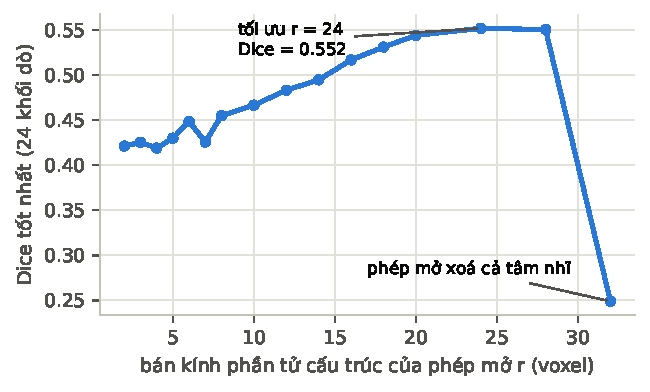
\includegraphics[width=0.55\linewidth]{classical_radius.pdf}
\caption{Pipeline cổ điển: Dice theo bán kính phép mở $r$ (mỗi điểm là bộ $(\sigma,k)$ tốt nhất đã thử với $r$ đó, trên 24 khối dò tham số).}
\label{fig:pp}
\end{figure}

\begin{table}[t]
\centering\small
\caption{Ảnh hưởng của hậu xử lý hình thái (cộng dồn từng bước) lên Dice và HD95 (voxel) trên tập test; 72 khối huấn luyện, trung bình 3 seed.}
\label{tab:pp}
\resizebox{\linewidth}{!}{\begin{tabular}{lcccccccccccc}
\toprule
Hậu xử lý & \multicolumn{2}{c}{U-Net} & \multicolumn{2}{c}{DINOv3} & \multicolumn{2}{c}{MRI-CORE} & \multicolumn{2}{c}{Ghép nối} & \multicolumn{2}{c}{GateFuse} & \multicolumn{2}{c}{D+}\\
 & Dice & HD95 & Dice & HD95 & Dice & HD95 & Dice & HD95 & Dice & HD95 & Dice & HD95\\
\midrule
Ngưỡng 0{,}5 & 0{,}912 & 8{,}22 & 0{,}902 & 11{,}02 & 0{,}908 & 7{,}82 & 0{,}912 & 8{,}13 & 0{,}911 & 7{,}43 & 0{,}913 & 7{,}52\\
+ TPLT lớn nhất & 0{,}913 & 6{,}69 & 0{,}905 & 7{,}90 & 0{,}909 & 6{,}70 & 0{,}913 & 7{,}04 & 0{,}912 & 6{,}24 & 0{,}914 & 6{,}54\\
+ lấp lỗ & 0{,}913 & 6{,}65 & 0{,}905 & 7{,}81 & 0{,}909 & 6{,}65 & 0{,}913 & 6{,}95 & 0{,}912 & 6{,}19 & 0{,}914 & 6{,}43\\
+ đóng & 0{,}914 & 6{,}32 & 0{,}908 & 7{,}10 & 0{,}910 & 6{,}47 & 0{,}915 & 6{,}76 & 0{,}914 & 5{,}82 & 0{,}915 & 6{,}15\\
\bottomrule
\end{tabular}}
\end{table}

\subsection{Phân tích định tính và bản đồ cổng}
Ở ca trung vị (Hình~\ref{fig:qual}), mọi phương pháp học đều bám sát nhãn và khác nhau chủ yếu ở nhánh tĩnh mạch phổi mảnh phía dưới. Ở ca khó nhất (tương phản thấp), GateFuse để lại một lỗ trong khoang (loại lỗi mà bước lấp lỗ xử lý được), còn D+ bám biên tốt hơn. Trên toàn tập test, \ErrBand\% số voxel sai nằm trong dải $\pm2$ voxel quanh biên, dù dải này chỉ chứa \RefBand\% thể tích tâm nhĩ; \ErrEnds\% số voxel sai nằm ở 20\% lát đầu/cuối của tâm nhĩ (vùng tĩnh mạch phổi và đáy nhĩ, chỉ chứa \RefEnds\% thể tích). Lỗi tập trung đúng ở những khó khăn cốt lõi đã nêu ở mục~1.

\textbf{RQ3} (Hình~\ref{fig:gate}). Cổng học được một phân công không gian rất rõ: bên trong tâm nhĩ $g=\GateInside$ (gần như chỉ dùng MRI-CORE), ở dải biên $g=\GateBoundary$, còn ở nền gần và nền xa $g$ lần lượt là \GateNear{} và \GateFar{} (nghiêng về DINOv3). Nói cách khác, mô hình dùng đặc trưng chuyên MRI để quyết định ``voxel này có phải máu trong tâm nhĩ không'' và dùng đặc trưng tổng quát để nắm ngữ cảnh hình dạng xung quanh, phù hợp với hình PCA ở Hình~\ref{fig:demo}.

\begin{figure}[t]
\centering
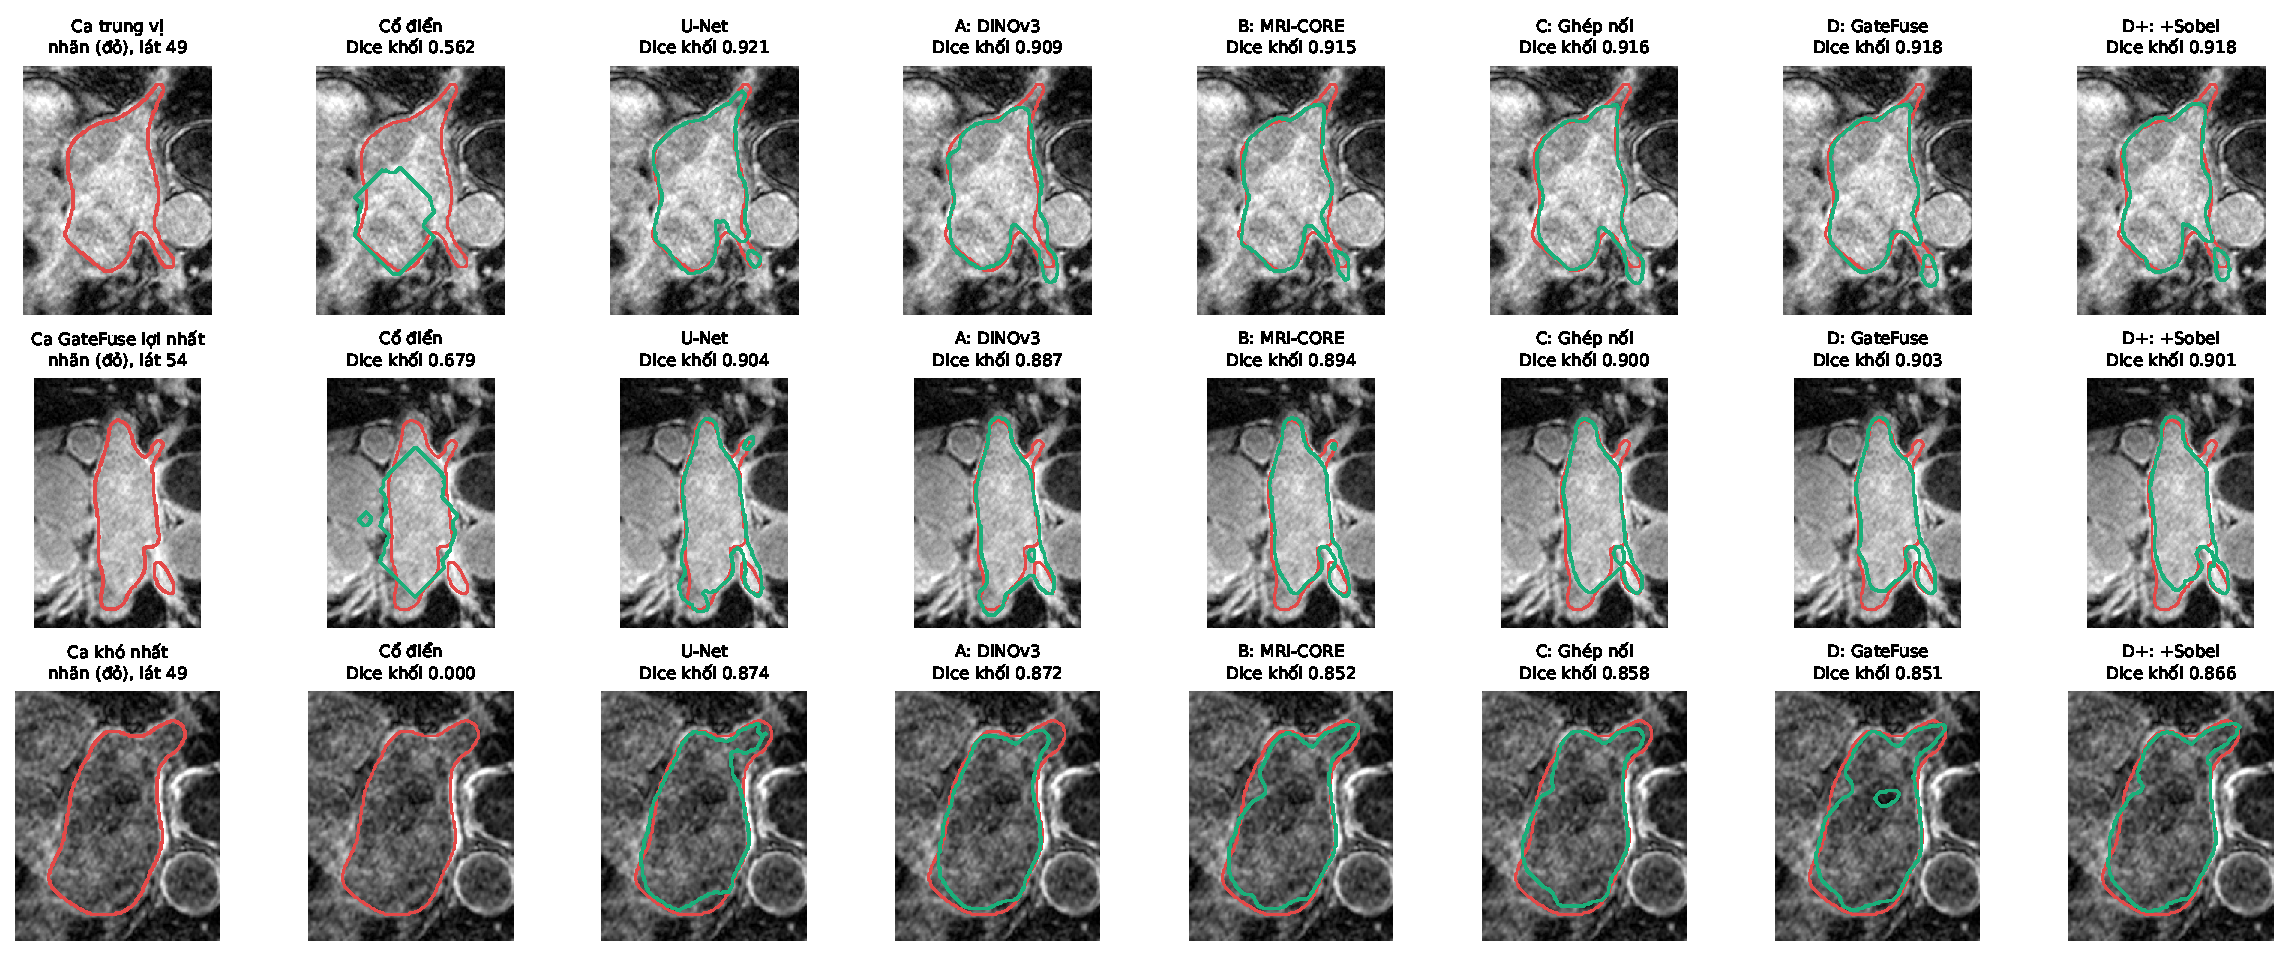
\includegraphics[width=\linewidth]{qualitative.pdf}
\caption{Ba ca test (lát có diện tích tâm nhĩ lớn nhất): ca có Dice trung vị theo GateFuse, ca GateFuse lợi nhất so với encoder đơn tốt hơn, và ca khó nhất. Đỏ: nhãn; xanh: dự đoán (seed 0, chưa hậu xử lý); tiêu đề ghi Dice của cả khối (trung bình 3 seed).}
\label{fig:qual}
\end{figure}

\begin{figure}[t]
\centering
\begin{minipage}[c]{0.62\linewidth}\centering
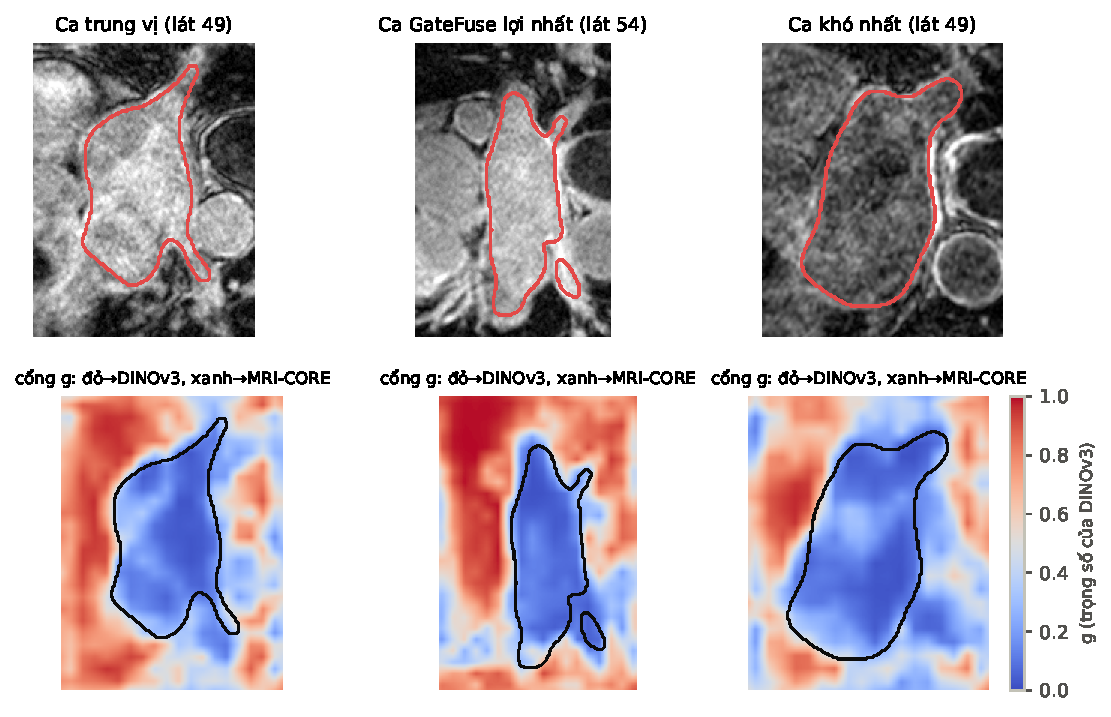
\includegraphics[width=\linewidth]{gate_maps.pdf}
\end{minipage}\hfill
\begin{minipage}[c]{0.36\linewidth}\centering
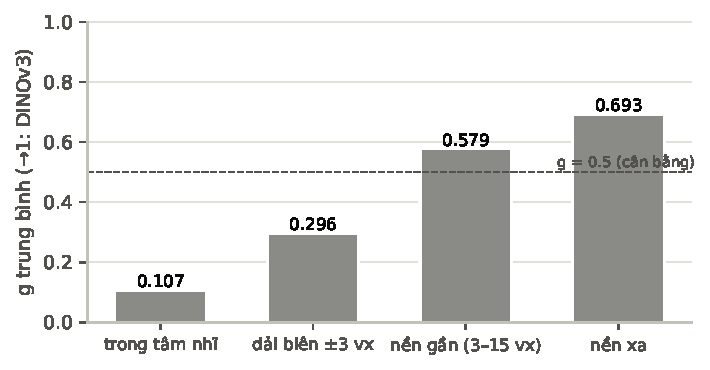
\includegraphics[width=\linewidth]{gate_regions.pdf}
\end{minipage}
\caption{Trái: bản đồ cổng $g$ của GateFuse trên ba ca ở Hình~\ref{fig:qual} (đỏ: tin DINOv3, xanh: tin MRI-CORE; viền đen: nhãn). Phải: giá trị $g$ trung bình theo vùng giải phẫu trên toàn bộ tập test (3 seed); vùng được xác định từ nhãn bằng phép giãn/co 3D (chương 7).}
\label{fig:gate}
\end{figure}

%-------------------------------------------------------------- 7
\section{Thảo luận}
\textbf{Trả lời câu hỏi nghiên cứu.} (RQ1) Có: dù mô tả dữ liệu tiền huấn luyện của MRI-CORE không nhắc tới tim, đặc trưng học trên MRI vẫn tốt hơn đặc trưng ảnh tự nhiên, rõ nhất ở biên. (RQ2) Có: hai loại đặc trưng bổ sung cho nhau. Ghép có cổng không hơn ghép nối về Dice, nhưng có HD95 tốt hơn khi đủ nhãn và đổi lại khả năng giải thích. (RQ3) MRI-CORE đảm nhận bên trong và biên, DINOv3 đảm nhận ngữ cảnh. (RQ4) Lợi thế của mô hình nền tảng nằm ở chế độ ít nhãn: hơn U-Net khoảng 3 điểm Dice và ổn định hơn nhiều giữa các seed; khi đủ 72 khối thì U-Net bắt kịp. (RQ5) Hậu xử lý hình thái rất rẻ (vài giây trên CPU) nhưng giảm HD95 17--36\%. Pipeline cổ điển thuần chỉ đạt \DiceClassicalFull{}: xử lý ảnh cổ điển hiệu quả nhất khi được dùng \emph{quanh} một bộ phân đoạn học được, chứ không thay thế nó.

\textbf{Đối chiếu tham khảo.} Trên cùng cách chia 80/20 của bộ dữ liệu này, tài liệu về học bán giám sát báo cáo: V-Net 3D học đủ 80 khối đạt Dice 91,14\%; chỉ 8 khối có nhãn đạt khoảng 79--80\%; UA-MT dùng thêm 72 khối không nhãn đạt 84,25\% \cite{uamt,jiao2022}. D+ đạt \DiceGateEdgeFull{} (72 khối) và \DiceGateEdgeFew{} (8 khối, \DicePpGateEdgeFew{} sau hậu xử lý) mà không dùng dữ liệu không nhãn. Đây chỉ là đối chiếu tham khảo: các tác giả dùng mạng 3D và quy trình chọn checkpoint khác, còn chúng tôi dùng thêm 8 khối có nhãn làm tập validation.

\textbf{Chi phí tính toán.} Nhờ đặc trưng được tính sẵn, một vòng huấn luyện của đầu GateFuse mất \TrainMsGate\,ms, so với \TrainMsUnet\,ms của U-Net (Apple M2 Pro, batch 16). Ngược lại, suy luận một khối 88 lát mất \InferGate\,s vì phải chạy hai ViT-B, so với \InferUnet\,s của U-Net. Mô hình nền tảng vì vậy phù hợp nhất khi nhãn khan hiếm và thời gian suy luận vài giây là chấp nhận được.

\textbf{Hạn chế.} (i) Vùng cắt sẵn của dữ liệu được lấy từ hộp bao của nhãn (quy ước của \cite{uamt}), nên bước định vị tâm nhĩ đã được bỏ qua cho mọi phương pháp; kết quả không so trực tiếp được với các thí nghiệm trên ảnh đầy đủ. (ii) Mô hình chạy theo từng lát 2D, encoder đông cứng và không dùng tăng cường dữ liệu; tinh chỉnh encoder (ví dụ LoRA) hoặc thêm ngữ cảnh 3D có thể cải thiện cả hai nhánh. (iii) Chỉ một bộ dữ liệu, một trung tâm; 3 seed và 20 ca test cho độ tin cậy thống kê vừa phải. (iv) Lưới vị trí của MRI-CORE được nội suy từ $14\times14$ (độ phân giải lúc tiền huấn luyện) lên $32\times32$, có thể chưa khai thác hết mô hình này.

\textbf{Hướng phát triển.} Kiểm định ngoài trên dữ liệu khác trung tâm; dùng D+ làm đầu vào cho học bán giám sát với 72 khối không nhãn; tinh chỉnh LoRA cho cả hai encoder; mở rộng cổng sang 3D để tận dụng tính liên tục giữa các lát.

%-------------------------------------------------------------- 8
\section{Kết luận}
Dự án đã xây dựng một pipeline năm bước (dữ liệu, tiền xử lý, phân đoạn, hậu xử lý, đánh giá) cho bài toán phân đoạn tâm nhĩ trái trên LGE-MRI, với đối chứng cổ điển và học sâu, 3 seed và kiểm định thống kê trên 20 khối test. Các kết quả chính:
(i) ghép đặc trưng tổng quát (DINOv3) với đặc trưng chuyên MRI (MRI-CORE) tốt hơn từng loại riêng;
(ii) cổng học được cho thấy rõ phân công: MRI-CORE cho bên trong tâm nhĩ, DINOv3 cho ngữ cảnh;
(iii) khi chỉ có 8 khối có nhãn, các đầu nhẹ trên đặc trưng nền tảng vượt U-Net học từ đầu khoảng 3 điểm Dice;
(iv) các bước xử lý ảnh cổ điển (kéo giãn tương phản, Sobel, phép mở/đóng, thành phần liên thông) vẫn đóng góp rõ rệt khi đặt quanh mô hình học.
Pipeline cuối (D+ và hậu xử lý) đạt Dice \DicePpGateEdgeFull{} với 72 khối và \DicePpGateEdgeFew{} với 8 khối có nhãn.

%-------------------------------------------------------------- 9
\section{Phân công công việc}
\begin{center}\small
\begin{tabularx}{\linewidth}{lX}
\toprule
Thành viên & Nhiệm vụ\\
\midrule
{[Họ tên SV1]} (trưởng nhóm) & Định vị bài toán, thiết kế GateFuse, tổng hợp báo cáo và slide\\
{[Họ tên SV2]} & Dữ liệu, tiền xử lý, phương pháp cổ điển (Otsu + hình thái) và dò tham số\\
{[Họ tên SV3]} & Trích đặc trưng DINOv3/MRI-CORE, huấn luyện các cấu hình A--D\\
{[Họ tên SV4]} & U-Net đối chứng, thí nghiệm ít nhãn, hậu xử lý hình thái\\
{[Họ tên SV5]} & Đánh giá, kiểm định thống kê, hình minh hoạ, demo và README\\
\bottomrule
\end{tabularx}
\end{center}

%-------------------------------------------------------------- 10
\section{Khai báo sử dụng AI}
Nhóm sử dụng trợ lý AI \textbf{Claude} (mô hình Claude Opus 5.5 của Anthropic, thông qua công cụ Claude Code) trong các việc sau: (i) thảo luận định vị lại bài toán và đề xuất thiết kế thí nghiệm (cấu hình A--D, đối chứng, kiểm định thống kê); (ii) viết mã nguồn Python trong thư mục \texttt{code/} (tiền xử lý, trích đặc trưng, huấn luyện, đánh giá, vẽ hình, demo); (iii) chạy toàn bộ thí nghiệm trên máy của nhóm và tổng hợp kết quả; (iv) soạn thảo báo cáo này và slide bằng LaTeX. Mọi con số trong báo cáo được sinh tự động từ kết quả chạy thật (\texttt{results/tables/}, tệp \texttt{numbers.tex}), không được nhập tay. Dữ liệu, trọng số MRI-CORE và DINOv3 là của các tác giả gốc và được trích dẫn đầy đủ. Nhóm chịu trách nhiệm đọc hiểu, kiểm tra lại mã nguồn, kết quả và nội dung trước khi nộp.

%-------------------------------------------------------------- refs
\begingroup\small
\begin{thebibliography}{99}\setlength{\itemsep}{1pt}
\bibitem{xiong2021} Z. Xiong và cs., ``A global benchmark of algorithms for segmenting the left atrium from late gadolinium-enhanced cardiac magnetic resonance imaging,'' \emph{Medical Image Analysis}, 67:101832, 2021.
\bibitem{uamt} L. Yu, S. Wang, X. Li, C.-W. Fu, P.-A. Heng, ``Uncertainty-aware self-ensembling model for semi-supervised 3D left atrium segmentation,'' MICCAI, 2019.
\bibitem{dinov3} O. Siméoni và cs., ``DINOv3,'' arXiv:2508.10104, 2025.
\bibitem{dinov2} M. Oquab và cs., ``DINOv2: Learning robust visual features without supervision,'' \emph{TMLR}, 2024.
\bibitem{mricore} H. Dong, Y. Chen, H. Gu, N. Konz, Y. Chen, Q. Li, M. A. Mazurowski, ``MRI-CORE: A foundation model for magnetic resonance imaging,'' arXiv:2506.12186, 2025.
\bibitem{liu2025dinov3med} C. Liu và cs., ``Does DINOv3 set a new medical vision standard?,'' arXiv:2509.06467, 2025.
\bibitem{adadino} Q. K. Be, N. H. Tran, G. D. T. Nguyen, Q. Dao Thi Thuy, ``AdaDINO-LA: A controlled study of DINOv2 adaptation strategies for left atrial segmentation in LGE-MRI,'' bản thảo, 2026. \url{https://github.com/qkhanhbe/AdaDINO-LA}
\bibitem{kundu2025} Kundu và cs., ``Multi-scale feature fusion with image-driven spatial integration for left atrium segmentation from cardiac MRI images,'' arXiv:2502.06615, 2025.
\bibitem{dsunet} ``DSU-Net: An improved U-Net model based on DINOv2 and SAM2 with multi-scale cross-model feature enhancement,'' arXiv:2503.21187, 2025.
\bibitem{jiao2022} R. Jiao và cs., ``Learning with limited annotations: a survey on deep semi-supervised learning for medical image segmentation,'' arXiv:2207.14191, 2022.
\bibitem{sam} A. Kirillov và cs., ``Segment Anything,'' ICCV, 2023.
\bibitem{unet} O. Ronneberger, P. Fischer, T. Brox, ``U-Net: Convolutional networks for biomedical image segmentation,'' MICCAI, 2015.
\bibitem{otsu} N. Otsu, ``A threshold selection method from gray-level histograms,'' \emph{IEEE Trans. SMC}, 9(1):62--66, 1979.
\bibitem{gonzalez} R. C. Gonzalez, R. E. Woods, \emph{Digital Image Processing}, 4th ed., Pearson, 2018.
\end{thebibliography}
\endgroup

\end{document}
